\chapter{触摸延时开关电路图}

{\bfseries 知识目标}
\begin{itemize}
\item 掌握AutoCAD图块的定义、使用方法
\item 掌握用AutoCAD绘制电路图的基本方法和步骤
\item 掌握电子元件的绘图方法和技巧
\end{itemize}

{\bfseries 技能目标}
\begin{itemize}
\item 具备绘制电子元器件的能力
\item 具备绘制电路图的能力
\end{itemize}

{\bfseries 本章导引}

本章我们将运用AutoCAD完成图\ref{fig:zhumodianlu}所示的触摸延时开关电路图项目的绘制,使读者掌握AutoCAD图块的定义和使用方法,了解运用AutoCAD绘制一般电路图的基本步骤、方法和技巧。读者通过学习本章的内容能够了解和掌握运用AutoCAD定制各种电气元件的规范和方法,实现具备绘制一般电路图的能力。
\noindent
\begin{figure}[htbp]
\centering
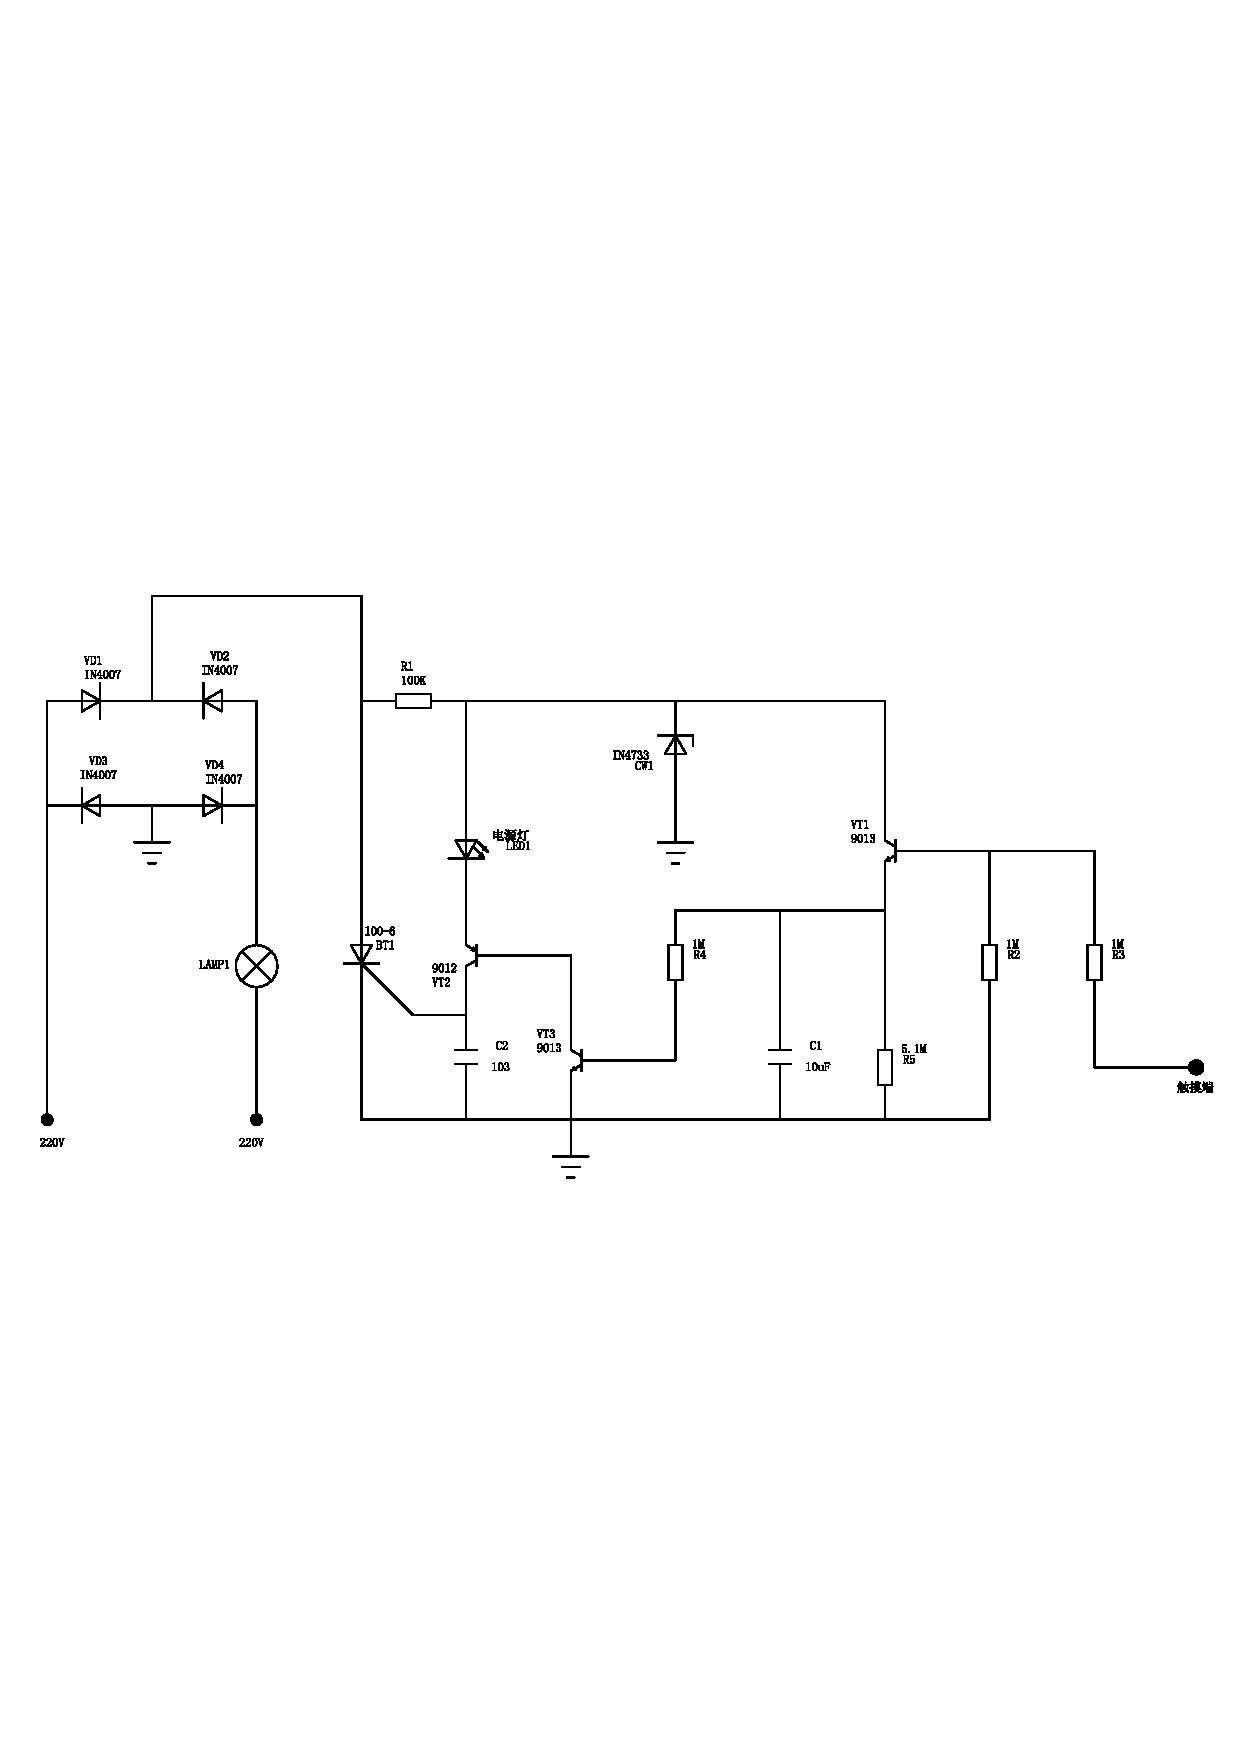
\includegraphics[scale=0.6]{zumoyanshidianlu.pdf}
\caption{触摸延时开关电路图}\label{fig:zhumodianlu}
\end{figure}
\indent

\endinput
